\documentclass{article}

% Language setting
\usepackage[english]{babel}

% Set page size and margins
\usepackage[letterpaper,top=2cm,bottom=2cm,left=3cm,right=3cm,marginparwidth=1.75cm]{geometry}

% Useful packages
\usepackage{amsmath}
\usepackage{graphicx}
\usepackage[hidelinks]{hyperref}

\title{Merapar Challenge}
\author{Pablo Cano}

\begin{document}
\maketitle

\section{Introduction}

This report explains the solution developed for the challenge of creating a web page with dynamic content. The implementation utilizes Terraform for Infrastructure as Code (IaC), AWS as the cloud provider, and Python for the application logic. Two distinct approaches were developed, each with different characteristics in terms of functionality and performance.

\section{Solution}

For this challenge, two different solutions were implemented using similar technologies but with different architectural approaches, resulting in varying performance characteristics.

\subsection{Static Hosting via S3}

This solution leverages the following AWS services. The proposed architecture is illustrated in Figure \autoref{fig:s3-diag}.

\begin{itemize}
    \item AWS Systems Manager Parameter Store: Stores the dynamic string with capability for console or programmatic updates
    \item S3 Bucket: Hosts the static web page content
    \item Lambda Function: Updates the index.html file in the S3 bucket when the parameter changes
    \item EventBridge Rule: Monitors changes to the SSM parameter and triggers the Lambda function
\end{itemize}

\begin{figure}[h]
\centering
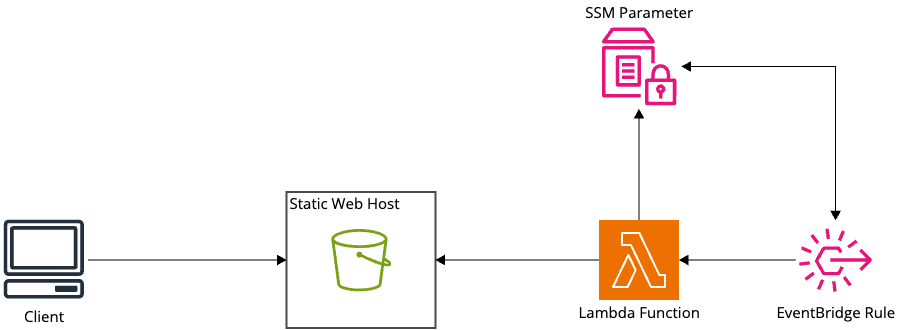
\includegraphics[width=0.8\textwidth]{s3-solution.png}
\caption{Architecture diagram of the S3 bucket solution.}
\label{fig:s3-diag}
\end{figure}

This solution provides a simple and straightforward implementation that demonstrates cloud capabilities effectively. However, it introduces some latency in content updates as changes propagate through the system.

\subsection{API Gateway with Dynamic Rendering}

This alternative solution employs server-side rendering through the following components:

\begin{itemize}
    \item AWS Systems Manager Parameter Store: Maintains the dynamic string content
    \item Lambda Function: Dynamically generates HTML content using the current SSM parameter value
    \item API Gateway: Serves as an HTTP endpoint with Lambda integration to handle web requests
\end{itemize}

The infrastructure for this approach is shown in Figure \autoref{fig:api-diag}.

\begin{figure}[h]
\centering
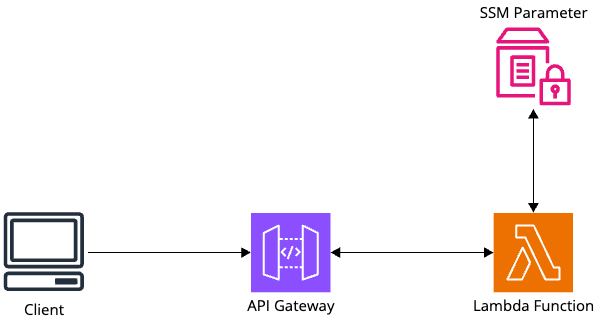
\includegraphics[width=0.8\textwidth]{api-solution.png}
\caption{Architecture diagram of the API Gateway solution.}
\label{fig:api-diag}
\end{figure}

This architecture eliminates the update latency of the S3 solution but requires rendering the web page for each incoming request, which impacts scalability for high-traffic scenarios.

\section{Discussion}

\subsection{Technology Selection}

The chosen technologies were selected based on simplicity, cost-effectiveness, and integration capabilities:

\begin{itemize}
    \item \textbf{SSM Parameter Store}: Provides parameter storage with versioning, multiple access methods, and native AWS service integration. The free tier for standard parameters makes it ideal for this solution. While AWS Secrets Manager offers similar functionality with automatic rotation, it lacks a free tier.
    
    \item \textbf{S3 Bucket}: Offers a cost-effective, scalable solution for static web hosting with robust versioning and access control capabilities. Alternatives like EC2 instances would introduce unnecessary complexity and cost, while AWS Amplify would be overly sophisticated for this simple use case.
    
    \item \textbf{Lambda}: Serves as the compute layer in both solutions due to its simplicity, automatic scaling, and native integration with other AWS services. While EC2, ECS Fargate, or similar services could be used, they would require additional infrastructure management and incur higher costs.
\end{itemize}

\subsection{Solution Comparison}

Both solutions successfully meet the challenge requirements but employ fundamentally different approaches:

\begin{itemize}
    \item \textbf{S3 Solution}:
    \begin{itemize}
        \item Pros: Highly cost-effective for infrequently changing content; efficient for high traffic scenarios
        \item Cons: Update latency between parameter changes and content visibility; less responsive to frequent changes
    \end{itemize}
    
    \item \textbf{API Gateway Solution}:
    \begin{itemize}
        \item Pros: Real-time content updates; immediate reflection of parameter changes
        \item Cons: Higher operational costs under heavy load; unnecessary computations for static content
    \end{itemize}
\end{itemize}

\subsection{Potential Improvements}

\begin{itemize}
    \item \textbf{S3 Solution Enhancements}:
    \begin{itemize}
        \item Implement CloudFront for global content delivery and HTTPS support, requiring distribution invalidation after each update
        \item Enhance the static page to fetch dynamic content client-side via API calls, though this would require additional authentication mechanisms
    \end{itemize}
    
    \item \textbf{API Gateway Solution Enhancements}:
    \begin{itemize}
        \item Implement caching mechanisms to reduce Lambda invocations for unchanged content
        \item Add a CDN layer to improve response times for geographically distributed users
        \item Consider provisioned concurrency to mitigate cold start latency issues
    \end{itemize}
    
    \item \textbf{General Improvements}:
    \begin{itemize}
        \item Implement monitoring and alerting for parameter changes and website availability
        \item Add authentication for parameter modification operations
        \item Implement CI/CD pipelines for infrastructure and code deployments
    \end{itemize}
\end{itemize}

\section{Conclusion}

Both solutions effectively address the challenge requirements while demonstrating different architectural patterns for dynamic web content. The S3-based solution excels in cost-efficiency for stable content with high traffic, while the API Gateway approach provides real-time updates at the expense of higher operational costs under load. The optimal choice depends on the specific use case parameters regarding change frequency and expected traffic patterns.

Future work could explore hybrid approaches combining the strengths of both solutions, such as implementing edge-optimized API endpoints with caching strategies to balance responsiveness and cost-efficiency.

\end{document}